\documentclass[12pt]{article}

\usepackage[utf8]{inputenc}
\usepackage{latexsym,amsfonts,amssymb,amsthm,amsmath}
\usepackage{tikz}
\usepackage{stanli}
\usetikzlibrary{shapes,calc,through,3d,patterns}
\usetikzlibrary{arrows.meta,decorations.pathreplacing,angles,quotes}
\usepackage{multicol}
\usepackage{geometry}
\usepackage{mathtools}
\usepackage{siunitx}
\usepackage{booktabs}
\usepackage{tabularx}


\setlength{\parindent}{0in}
\setlength{\oddsidemargin}{-0.25in}
\setlength{\textwidth}{7in}
\setlength{\textheight}{9.3in}
\setlength{\topmargin}{-1in}
\setlength{\headheight}{18pt}

\newcommand\blfootnote[1]{%
    \begingroup
    \renewcommand\thefootnote{}\footnote{#1}%
    \addtocounter{footnote}{-1}%
    \endgroup
}

\definecolor{darkred}{rgb}{0.6,0,0}

\newcommand{\bolddelta}{\boldsymbol\delta}
\newcommand{\boldxi}{\boldsymbol\xi}

\newcolumntype{M}[1]{>{\centering\arraybackslash}m{#1}}


\begin{document}


\noindent ME473 - Dynamic finite element analysis of structures\hfill EPFL\\
Stefano Burzio \hfill 2025\\
\vspace{0.3cm}

\hspace*{\fill}\textbf{\Large Final exam - solutions}\hspace*{\fill}

\hrulefill



\subsection*{Barème}
\textbf{Problem 1}
\begin{itemize}
	\item[(a)] Constrained DOFs 1pt, unconstrained DOFs 1pt
	\item[(b)] Elementary matrices 2pts, assembly 3p, reducing and boundary conditions 1pt
	\item[(c)] Computing determinant 1pt, solving characteristic equation ($lambda_i$) 2 pts, $w_i=\sqrt{\lambda_i}$ 1pt, first eigenvector 1pt, interpretation 1pt
	\item[(d)] Max $E/rho$ 1 pt, justification 1 pt
	\item[(e)] $K$ and $M$ 1p, $q$ 1 pt, ODE system 1 pt, solving the ODEs 2pts, resonance 1pt
	\item[(f)] Sketch 1pt, justification 2pts
\end{itemize}
\textbf{Problem 2}
\begin{itemize}
	\item[(a)] Strong form 4pts, Ipp 1pt, weak form 1pt
	\item[(b)] Components of ${}^1T$ 2 pts, Jacobian matrix and determinant 1pt
	\item[(c)] -1pt if one mistake, -2pts if 2 mistakes
	\item[(d)] Expression of $M$ 2pts, $M_{12}$ 1pt, $M_{12}$ 1pt
	\item[(e)] Bounds on error 2pts, justification 2pts
	\item[(f)] jacobian 1pt, shape function matrix 1pt, order 7 thus 4x4 1pt, $K$ 1pt
	\item[(g)] implicit 1pt, justification average acceleration 1pt
\end{itemize}

\newpage
\subsection*{Problem 1}
\paragraph*{(a) Degree of freedom classification.} Each node in a 2D truss structure has two degrees of freedom: horizontal ($q_{ix}$) and vertical ($q_{iy}$) displacements. There are 4 nodes, thus $8$ total DOFs. We now apply the boundary conditions:
\begin{itemize}
	\item Nodes 1 and 4 are fixed $\Rightarrow$ $q_{1x} = q_{1y} = 0$ and $q_{4x} = q_{4y} = 0$,
	\item Node 2 rests on a roller support $\Rightarrow$ $q_{2y}= 0$ but $q_{2x}$ is free.
\end{itemize}
Thus, the constrained DOFs are: $q_{1x}, q_{1y}, q_{2y}, q_{4x}, q_{4y}$, the unconstrained DOFs are: \(q_{2x}, q_{3x}, q_{3y}\).

\paragraph*{(b) Element matrices and assembly.} Recall that for a generic truss element:
\[
	^{e}\mathbf{K} = \frac{{}^{e}E{}^{e}A}{^{e}\ell}
	\begin{bmatrix}
		c^2  & cs   & -c^2 & -cs  \\
		cs   & s^2  & -cs  & -s^2 \\
		-c^2 & -cs  & c^2  & cs   \\
		-cs  & -s^2 & cs   & s^2
	\end{bmatrix},\qquad
	^{e}\mathbf{M} = \frac{^{e}\rho ^{e}A ^{e}\ell}{6}
	\begin{bmatrix}
		2c^2 & 2cs  & c^2  & cs   \\
		2cs  & 2s^2 & cs   & s^2  \\
		c^2  & cs   & 2c^2 & 2cs  \\
		cs   & s^2  & 2cs  & 2s^2
	\end{bmatrix}
\]
where $c=\cos({}^e\theta)$ and $s=\sin({}^e\theta)$. For the considered structure, the following applies:
\begin{table}[h!]
	\centering
	\begin{tabular}{|c|c|c|c|ll|}
		\hline
		\textbf{Element} & \textbf{Nodes} & \textbf{Length ${}^e\ell$ (m)} & \multicolumn{3}{|c|}{\textbf{Orientation ${}^e\theta$ }}                                                       \\
		\hline
		1                & 1–2            & 3                              & Horizontal                                               & $\cos({}^1\theta) = 1$    & $\sin({}^1\theta) = 0$  \\
		2                & 2–3            & 4                              & Vertical                                                 & $\cos({}^2\theta) = 0$    & $\sin({}^2\theta) = 1$  \\
		3                & 1–3            & 5                              & Diagonal                                                 & $\cos({}^3\theta)  = 3/5$ & $\sin({}^3\theta) =4/5$ \\
		4                & 3–4            & 3                              & Horizontal                                               & $\cos({}^4\theta) = 1$    & $\sin({}^4\theta) = 0$  \\
		\hline
	\end{tabular}
\end{table}

Although the problem specifically requests the elementary1 stiffness matrices, we include the mass matrices as well for completeness.

\begin{minipage}{0.48\textwidth}
	\begin{align*}
		{}^1\mathbf K ={}^4\mathbf K & =\frac{EA}{3}\begin{bmatrix}
			                                            1  & 0 & -1 & 0 \\
			                                            0  & 0 & 0  & 0 \\
			                                            -1 & 0 & 1  & 0 \\
			                                            0  & 0 & 0  & 0 \\
		                                            \end{bmatrix} \\
		{}^2\mathbf K                & =\frac{EA}{4}\begin{bmatrix}
			                                            0 & 0  & 0 & 0  \\
			                                            0 & 1  & 0 & -1 \\
			                                            0 & 0  & 0 & 0  \\
			                                            0 & -1 & 0 & 1  \\
		                                            \end{bmatrix} \\
		{}^3\mathbf K                & =EA\begin{bmatrix}
			                                  9   & 12  & -9  & -12 \\
			                                  12  & 16  & -12 & -16 \\
			                                  -9  & -12 & 9   & 12  \\
			                                  -12 & -16 & 12  & 16  \\
		                                  \end{bmatrix}
	\end{align*}
\end{minipage}
\hfill
\begin{minipage}{0.48\textwidth}
	\begin{align*}
		{}^1\mathbf M ={}^4\mathbf M & =\frac{\rho A}{2}\begin{bmatrix}
			                                                2 & 0 & 1 & 0 \\
			                                                0 & 0 & 0 & 0 \\
			                                                1 & 0 & 2 & 0 \\
			                                                0 & 0 & 0 & 0 \\
		                                                \end{bmatrix}    \\
		{}^2\mathbf M                & =\frac{2\rho A}{3}\begin{bmatrix}
			                                                 0 & 0 & 0 & 0 \\
			                                                 0 & 2 & 0 & 1 \\
			                                                 0 & 0 & 0 & 0 \\
			                                                 0 & 1 & 0 & 2 \\
		                                                 \end{bmatrix}   \\
		{}^3\mathbf M                & =\frac{\rho A}{6}\begin{bmatrix}
			                                                18 & 24 & 9  & 12 \\
			                                                24 & 32 & 12 & 16 \\
			                                                9  & 12 & 18 & 24 \\
			                                                12 & 16 & 24 & 32 \\
		                                                \end{bmatrix}
	\end{align*}
\end{minipage}
\vspace{0.3cm}

Let's now assemble and write explicitly the global $8 \times 8$ stiffness and mass matrices $\mathbf{K}$ and $\mathbf{M}$:
\[
	\mathbf{K} =
	EA
	\begin{bmatrix}
		\frac{1}{3} + 9 & 12  & -\frac{1}{3} & 0           & -9              & -12              & 0            & 0 \\[5pt]
		12              & 16  & 0            & 0           & -12             & -16              & 0            & 0 \\[5pt]
		-\frac{1}{3}    & 0   & \frac{1}{3}  & 0           & 0               & 0                & 0            & 0 \\[5pt]
		0               & 0   & 0            & \frac{1}{4} & 0               & -\frac{1}{4}     & 0            & 0 \\[5pt]
		-9              & -12 & 0            & 0           & 9 + \frac{1}{3} & 12               & -\frac{1}{3} & 0 \\[5pt]
		-12             & -16 & 0            & \frac{1}{4} & 12              & 16 + \frac{1}{4} & 0            & 0 \\[5pt]
		0               & 0   & 0            & 0           & -\frac{1}{3}    & 0                & \frac{1}{3}  & 0 \\[5pt]
		0               & 0   & 0            & 0           & 0               & 0                & 0            & 0
	\end{bmatrix}
\]
and
\[
	\mathbf{M} = \rho A
	\begin{bmatrix}
		1 + \frac{18}{6} & \frac{24}{6} & \frac{1}{2} & 0           & \frac{9}{6}     & \frac{12}{6}               & 0           & 0 \\[5pt]
		\frac{24}{6}     & \frac{32}{6} & 0           & 0           & \frac{12}{6}    & \frac{16}{6}               & 0           & 0 \\[5pt]
		\frac{1}{2}      & 0            & 1           & 0           & 0               & 0                          & 0           & 0 \\[5pt]
		0                & 0            & 0           & \frac{4}{3} & 0               & \frac{2}{3}                & 0           & 0 \\[5pt]
		\frac{9}{6}      & \frac{12}{6} & 0           & 0           & \frac{18}{6}+ 1 & \frac{24}{6}               & \frac{1}{2} & 0 \\[5pt]
		\frac{12}{6}     & \frac{16}{6} & 0           & \frac{4}{3} & \frac{24}{6}    & \frac{32}{6} + \frac{2}{3} & 0           & 0 \\[5pt]
		0                & 0            & 0           & 0           & \frac{1}{2}     & 0                          & 1           & 0 \\[5pt]
		0                & 0            & 0           & 0           & 0               & 0                          & 0           & 0
	\end{bmatrix}
\]
After assembling the global stiffness $\mathbf{K}$ and mass $\mathbf{M}$ matrices and eliminating the constrained DOFs, corresponding to rows and columns indexed by 1, 2, 4, 7 and 8, the reduced matrices corresponding to the three free DOFs $q_{2x}, q_{3x}, q_{3y}$ are:
\[
	\mathbf K_{red}=EA\begin{bmatrix}
		1/3 & 0    & 0    \\
		0   & 28/3 & 12   \\
		0   & 12   & 65/4 \\
	\end{bmatrix}, \quad\text{and}\quad
	\mathbf{M}_{red}=\rho A\begin{bmatrix}
		1 & 0 & 0 \\
		0 & 4 & 4 \\
		0 & 4 & 6 \\
	\end{bmatrix}.
\]

\paragraph*{(c) Lowest natural frequencies.} To determine the natural frequencies and mode shapes of the structure, we solve the generalized eigenvalue problem:
\[
	\mathbf{K}_{\text{red}} \, \mathbf{p} = \lambda\, \mathbf{M}_{\text{red}} \, \mathbf{p},
\]
where \( \omega=\sqrt{\lambda} \) is the natural circular frequency and \( \mathbf p \) is the associated mode shape. We solve $\text{det}\left(\mathbf{K}_{red}  - \lambda \mathbf{M}_{red}\right)=0$ assuming normalized parameters: \( E = A = \rho = 1 \), that leads to
\begin{align*}
	\text{det}\left(\begin{bmatrix}
			                1/3 & 0    & 0    \\
			                0   & 28/3 & 12   \\
			                0   & 12   & 65/4 \\
		                \end{bmatrix}-\lambda\begin{bmatrix}
			                                     1 & 0 & 0 \\
			                                     0 & 4 & 4 \\
			                                     0 & 4 & 6 \\
		                                     \end{bmatrix}\right)                                                  & =0, \\
	\left(\frac{1}{3}-\lambda\right)\left(8 \lambda^2 - 25 \lambda + \frac{23}{3} \right) & = 0.
\end{align*}
This leads to three eigenvalues:
\begin{align*}
	\lambda_1 & = \omega_1^2 = \frac{1}{3},                                           \\
	\lambda_2 & = \omega_2^2 = \frac{1}{16}\left(25-\sqrt\frac{1139}{3}\right)=0.345, \\
	\lambda_3 & = \omega_3^2 = \frac{1}{16}\left(25+\sqrt\frac{1139}{3}\right)=2.780.
\end{align*}


Thus, the lowest two natural frequencies are: $\omega_1 \approx 0.577$, $\omega_2  \approx 0.587$ and $\omega_3  \approx 1.667$. The first eigenvector (mode shape) is simply:
\[
	\mathbf p_1 = \begin{bmatrix} 1 \\ 0 \\ 0 \end{bmatrix}, \quad
\]
This indicates that in the first mode, the transverse displacement of node 2 dominates and the displacement of node 3 is negligible.


\paragraph*{(d) Maximizing fundamental frequency.} To maximize the fundamental frequency of a structure, one must maximize the ratio of stiffness to mass. The fundamental (circular) frequency \( \omega_1 \) of a structure is approximately given by:
\[
	\omega_1 \approx \sqrt{\frac{k_{\text{eff}}}{m_{\text{eff}}}} \propto \sqrt{\frac{EA}{\rho A}} = \sqrt{\frac{E}{\rho}},
\]
From this expression, we can derive the following design guidelines:
\begin{itemize}
	\item Maximize \( E \): selecting materials with a high Young's modulus (e.g., carbon fiber, titanium, steel) increases the stiffness and thus the frequency.
	\item Minimize \( \rho \): a lower mass density reduces the effective mass, thereby increasing the frequency. Materials with high stiffness-to-weight ratio (e.g., advanced composites) are ideal.
	\item Area \( A \): increasing the area \( A \) will note contributes to increasing the fundamental frequency.
\end{itemize}
To achieve the highest possible fundamental frequency, one should select materials with a high \( E/\rho \) ratio: high stiffness and low density.

\paragraph*{(e) Transient response and resonance under harmonic loading.}  Node 3 is constrained to move only in the vertical direction. Consequently, the degrees of freedom reduce to two: $\mathbf{q}_r(t)=[q_{2x}(t),\ q_{3y}(t)]^T$. Moreover, the structure is initially at rest:
\[
	\mathbf{q}_r(0) = \dot{\mathbf{q}_r}(0) = \mathbf{0}.
\]
The semi-discrete equation of motion is:
\[
	\mathbf{M}_r \ddot{\mathbf{q}}_r(t) + \mathbf{K}_r \mathbf{q}_r(t) = \mathbf{f}_r(t)
\]
where, assuming normalized parameters \( E = A = \rho = 1 \), we have
\[
	\mathbf{K}_r =\begin{bmatrix}
		1/3 & 0    \\
		0   & 65/4 \\
	\end{bmatrix} \qquad\text{and}\qquad \mathbf{M}_r=\begin{bmatrix}
		1 & 0 \\
		0 & 6 \\
	\end{bmatrix}.
\]
The harmonic vertical load \( f(t) = a \sin(\bar{\omega} t) \) is applied at node 3, thus the force vector is:
\[
	\mathbf{f}_r(t) =
	\begin{bmatrix}
		0                      \\
		a \sin(\bar{\omega} t) \\
	\end{bmatrix}.
\]
In general, we should express the solution as a linear combination of mode shapes:
\[
	\mathbf{q}_r(t) = z_1(t) {\mathbf p}_1 + z_2(t) {\mathbf p}_2,
\]
where \( {\mathbf p}_1 = \begin{bmatrix} 1 \\ 0 \end{bmatrix} \), \( {\mathbf p}_2 = \begin{bmatrix} 0 \\ 1 \end{bmatrix} \). However, the equation of motions are already decoupled. This leads to two uncoupled scalar second-order ordinary differential equations:
\begin{align*}
	\ddot{q}_{2x}(t) + \frac{1}{3} q_{2x} (t)     & = 0,                      \\
	6 \ddot{q}_{3y}(t) + \frac{65}{4}  q_{3y} (t) & =  a \sin(\bar{\omega} t)
\end{align*}
The initial conditions are \( q_{2x}(0) =  q_{3y}(0) = \dot{q}_{2x}(0) = \dot{q}_{3y}(0) = 0 \).
\begin{itemize}
	\item For \( q_{3y}(t) \): standard forced vibration response: let $\omega=\sqrt{\frac{65}{24}}$, then
	      \[
		      q_{3y}(t) = \frac{a}{6(\omega^2 - \bar{\omega}^2)}
		      \left( \sin(\bar{\omega} t) - \frac{\bar{\omega}}{\omega} \sin(\omega t) \right)
		      \quad \text{(for } \omega \neq \bar{\omega})
	      \]
	\item For \( q_{2x}(t) \): homogeneous solution:
	      \[
		      q_{2x}(t) = 0
	      \]
	\item Total response:
	      \[
		      \mathbf{q}_r(t) = \frac{a}{6(\omega^2 - \bar{\omega}^2)}
		      \left( \sin(\bar{\omega} t) - \frac{\bar{\omega}}{\omega} \sin(\omega t) \right)
		      \begin{bmatrix} 0 \\ 1 \end{bmatrix}
	      \]
\end{itemize}
Resonance occurs when the excitation frequency \( \bar{\omega} \) matches any of the system's natural frequencies. That means $\bar{\omega} = \omega$.

\paragraph*{(f) Rigid body mode.} For example:
\begin{center}
	\begin{minipage}{0.3\textwidth}
		\centering
		\begin{tikzpicture}
			\coordinate (1) at (0,0);
			\coordinate (2) at (3,0);
			\coordinate (3) at (3,4);
			\coordinate (4) at (0,4);
			\point{a}{0}{0};
			\point{b}{0}{4};
			\point{c}{3}{0};
			\point{d}{3}{4};
			\support{1}{a}[-90];
			\support{1}{b}[-90];
			\draw[ultra thick] (1) -- (2);
			\draw[ultra thick] (3) -- (4);
			\draw[ultra thick] (2) -- (3);
			\draw[thick,fill=white] (3) circle (3pt);
			\draw[thick,fill=white] (2) circle (3pt);
			\draw[thick,fill=white] (1) circle (3pt);
			\draw[thick,fill=white] (4) circle (3pt);
		\end{tikzpicture}
	\end{minipage}
	\hfill
	\begin{minipage}{0.3\textwidth}
		\centering
		\begin{tikzpicture}
			\coordinate (1) at (0,0);
			\coordinate (2) at (3,0);
			\coordinate (3) at (3,4);
			\coordinate (4) at (0,4);
			\point{a}{0}{0};
			\point{b}{0}{4};
			\point{c}{3}{0};
			\point{d}{3}{4};
			\support{2}{c};
			\support{2}{a};
			\support{1}{b}[-90];
			\draw[ultra thick] (1) -- (2);
			\draw[ultra thick] (3) -- (4);
			\draw[ultra thick] (2) -- (3);
			\draw[thick,fill=white] (3) circle (3pt);
			\draw[thick,fill=white] (2) circle (3pt);
			\draw[thick,fill=white] (1) circle (3pt);
			\draw [thick] (2.70,-0.55) circle [radius=0.05];
			\draw [thick] (3.00,-0.55) circle [radius=0.05];
			\draw [thick] (3.30,-0.55) circle [radius=0.05];
			\draw [thick] (-0.30,-0.55) circle [radius=0.05];
			\draw [thick] (0.00,-0.55) circle [radius=0.05];
			\draw [thick] (0.30,-0.55) circle [radius=0.05];
		\end{tikzpicture}
	\end{minipage}
	\hfill
	\begin{minipage}{0.3\textwidth}
		\centering
		\begin{tikzpicture}
			\coordinate (1) at (0,0);
			\coordinate (2) at (3,0);
			\coordinate (3) at (3,4);
			\coordinate (4) at (0,4);
			\point{a}{0}{0};
			\point{b}{0}{4};
			\point{c}{3}{0};
			\point{d}{3}{4};
			\support{1}{a}[-90];
			\support{1}{c}[0];
			\draw[ultra thick] (1) -- (2);
			\draw[ultra thick] (3) -- (1);
			\draw[ultra thick] (2) -- (3);
			\draw[ultra thick] (3) -- (4);
			\draw[thick,fill=white] (3) circle (3pt);
			\draw[thick,fill=white] (2) circle (3pt);
			\draw[thick,fill=white] (1) circle (3pt);
			\draw[thick,fill=white] (4) circle (3pt);
		\end{tikzpicture}
	\end{minipage}
\end{center}

\newpage
\subsection*{Problem 2}
\paragraph*{(a) Strong and weak forms.} Under the assumptions of plane stress, linear elasticity, and small deformations, the strong form of the dynamic equilibrium equations reads: find $\mathbf u\in C^2(\bar \Omega\times[0,T],\mathbb R^2)$ such that
$$ \nabla^T\mathbf C\nabla\mathbf u = \rho \ddot{\mathbf u}
	\qquad \text{or}\qquad \begin{cases}
		\partial_{x_1}\sigma_{11} + \partial_{x_2}\sigma_{12}  = \rho \ddot{u_{1}} \\
		\partial_{x_2}\sigma_{22} + \partial_{x_1}\sigma_{12}  = \rho \ddot{u_{2}}
	\end{cases},$$
coupled with boundary and initial conditions:
\[
	\begin{cases}
		\mathbf{u} = \mathbf{0}                     & \text{on } \Gamma_u = \overline{AB},                                              \\
		\mathbf N^T\boldsymbol{\sigma} = \mathbf{t} & \text{on } \Gamma_{\sigma_1} = \overline{CD},                                     \\
		\mathbf N^T\boldsymbol{\sigma} = \mathbf{0} & \text{on } \Gamma_{\sigma_2}=\partial\Omega\setminus(\Gamma_u\cup \Gamma_\sigma), \\
	\end{cases}
	\qquad\qquad
	\begin{cases}
		\mathbf u = \mathbf u_0       & \text{on } \Omega \text{ and } t=0, \\
		\dot{\mathbf u} = \mathbf v_0 & \text{on } \Omega \text{ and } t=0, \\
	\end{cases}
\]
where:
\begin{itemize}
	\item \( \mathbf{u} = \begin{bmatrix} u_1 \\ u_2 \end{bmatrix} \) is the displacement vector field;
	\item \( \boldsymbol{\sigma}= \begin{bmatrix} \sigma_{11} \\ \sigma_{22} \\ \sigma_{12} \end{bmatrix} \) is the Cauchy stress tensor in plane stress;
	\item $\nabla=\begin{bmatrix} \partial_{x_1} & 0 \\ 0 & \partial_{x_2} \\ \partial_{x_2} & \partial_{x_1}  \end{bmatrix}$ is the differential operator for plane stress.
	\item \( \mathbf{t} = \begin{bmatrix} q \\ 0 \end{bmatrix} \) is the applied traction vector on \( \overline{CD} \);
	\item \( \mathbf{n} = \begin{bmatrix} 0 \\ 1 \end{bmatrix} \) is the outward unit normal on \( \Gamma_\sigma \) and $\mathbf{N}^T=\begin{bmatrix}0 & 0 & 1 \\ 0 & 1 & 0\end{bmatrix}$. Thus
	      $$\mathbf{N}^T\boldsymbol{\sigma}=\begin{bmatrix}\sigma_{12} \\\sigma_{22} \end{bmatrix}$$
	\item  \( \mathbf{C} \) is the \( 3 \times 3 \) elasticity matrix for plane stress:
	      \[
		      \mathbf{C} =
		      \frac{E}{1 - \nu^2}
		      \begin{bmatrix}
			      1   & \nu & 0                 \\
			      \nu & 1   & 0                 \\
			      0   & 0   & \frac{1 - \nu}{2}
		      \end{bmatrix}.
	      \]
\end{itemize}
Multiply the strong form by a virtual displacement \( \boldsymbol{\delta u} \in \mathcal{V} \), integrate over \( \Omega \), and apply integration by parts:
\[
	\int_{\Omega} (\nabla \boldsymbol{\delta u})^T \mathbf{C} \nabla \mathbf{u}\;d\Omega
	+ \int_{\Omega} \rho \boldsymbol{\delta u}^T \ddot{\mathbf{u}} \; d\Omega
	= \int_{\Gamma_{\sigma_1}} \boldsymbol{\delta u}^T \mathbf{t} \; d\Gamma.
\]
Functional spaces:
\[
	\mathcal{U} = \{ \mathbf{u}(\cdot,t) \in H^1(\Omega,\mathbb R^2) \;:\; \mathbf{u}(\cdot,t) = \mathbf{0} \text{ on } \Gamma_u \}, \qquad
	\mathcal{V} = \{ \boldsymbol{\delta u} \in H^1(\Omega,\mathbb R^2) \;:\; \boldsymbol{\delta u} = \mathbf{0} \text{ on } \Gamma_u \}.
\]
We provide below some more details on how the weak form is derived from the strong form. Consider the first of the two equations in the strong form and apply the usual routine:
\begin{align*}
	\int_\Omega(\partial_{x_1}\sigma_{11} + \partial_{x_2}\sigma_{12})\delta u_1\, d\Omega                                                                                                                             & = \int_\Omega\rho \ddot{u_{1}}\delta u_1\ d\Omega  \\
	-\int_\Omega\sigma_{11}\partial_{x_1}\delta u_1 +\sigma_{12} \partial_{x_2}\delta u_1\ d\Omega + \int_{\partial\Omega}n_1\sigma_{11}\delta u_1\, d\Gamma + \int_{\partial\Omega}n_2\sigma_{12}\delta u_1\, d\Gamma & = \int_\Omega\rho \ddot{u_{1}}\delta u_1\, d\Omega \\
\end{align*}
Recall that $\partial\Omega=\Gamma_u\cap\Gamma_{\sigma_1}\cap \Gamma_{\sigma_2}$. On $\Gamma_u$ we have $\delta u_1=0$. On $\Gamma_{\sigma_1}$  we have $\sigma_{12}=q$ and $\sigma_{22}=0$ and $n_1=0$, $n_2=1$. On $\Gamma_{\sigma_2}$  we have
$$\mathbf{N}^T\boldsymbol{\sigma}=\begin{bmatrix}n_1\sigma_{11}+n_2\sigma_{12} \\n_2\sigma_{22}+n_1\sigma_{12} \end{bmatrix}=\begin{bmatrix}
		0 \\ 0
	\end{bmatrix}$$
Thus
$$\int_{\partial\Omega}n_1\sigma_{11}\delta u_1+n_2\sigma_{12}\delta u_1\, d\Gamma = \int_{\partial\Gamma_{\sigma_1}}q\delta u_1 \, d\Gamma = \int_{\Gamma_{\sigma_1}} \boldsymbol{\delta u}^T \mathbf{t} \; d\Gamma$$
Same argument applies for the second equation in the strong form:
\begin{align*}
	\int_\Omega(\partial_{x_2}\sigma_{22} + \partial_{x_1}\sigma_{12})\delta u_2\, d\Omega                                                                                                                             & = \int_\Omega\rho \ddot{u_{2}}\delta u_2\ d\Omega  \\
	-\int_\Omega\sigma_{22}\partial_{x_2}\delta u_2 +\sigma_{12} \partial_{x_1}\delta u_2\ d\Omega + \int_{\partial\Omega}n_2\sigma_{22}\delta u_2\, d\Gamma + \int_{\partial\Omega}n_1\sigma_{12}\delta u_2\, d\Gamma & = \int_\Omega\rho \ddot{u_{2}}\delta u_2\, d\Omega \\
\end{align*}
For the boundary terms we obtain:
$$\int_{\partial\Omega}n_2\sigma_{22}\delta u_2+n_1\sigma_{12}\delta u_2\, d\Gamma =  0$$
Notice that:
$$\int_\Omega\sigma_{11}\partial_{x_1}\delta u_1 +\sigma_{12} \partial_{x_2}\delta u_1 + \sigma_{22}\partial_{x_2}\delta u_2 +\sigma_{12} \partial_{x_1}\delta u_2\ d\Omega =\int_{\Omega} (\nabla \boldsymbol{\delta u})^T \boldsymbol{\sigma}\;d\Omega=\int_{\Omega} (\nabla \boldsymbol{\delta u})^T \mathbf{C} \nabla \mathbf{u}\;d\Omega$$
and
$$\int_\Omega\rho \ddot{u_{1}}\delta u_1 + \rho \ddot{u_{2}}\delta u_2\, d\Omega = \int_{\Omega} \rho \boldsymbol{\delta u}^T \ddot{\mathbf{u}} \; d\Omega$$
\paragraph*{(b) Transformation ${}^1T$.} We consider element \( {}^1\Omega \), whose nodes are:
\[
	\text{Node 1: } (x_1, y_1) = (0, 0), \quad
	\text{Node 5: } (x_2, y_2) = (20, 0), \quad
	\text{Node 4: } (x_3, y_3) = (5, 30).
\]
The reference triangle \( {}^a\Omega \) is defined in coordinates \( (\xi_1, \xi_2) \), with vertices: $(0,0)$, $(1,0)$, and $(0,1)$. The physical coordinates \( (x,y) \) are obtained from the reference coordinates \( (\xi_1, \xi_2) \) using the standard linear mapping:
\[
	\begin{bmatrix}
		x(\xi_1, \xi_2) \\
		y(\xi_1, \xi_2)
	\end{bmatrix}
	=
	(1 - \xi_1 - \xi_2)
	\begin{bmatrix}
		x_1 \\
		y_1
	\end{bmatrix}
	+
	\xi_1
	\begin{bmatrix}
		x_2 \\
		y_2
	\end{bmatrix}
	+
	\xi_2
	\begin{bmatrix}
		x_3 \\
		y_3
	\end{bmatrix}.
\]
Substituting the nodal coordinates of \( {}^1\Omega \):
\[
	\begin{aligned}
		x(\xi_1, \xi_2) & = (1 - \xi_1 - \xi_2)\cdot 0 + \xi_1 \cdot 20 + \xi_2 \cdot 5 = 20\xi_1 + 5\xi_2, \\
		y(\xi_1, \xi_2) & = (1 - \xi_1 - \xi_2)\cdot 0 + \xi_1 \cdot 0 + \xi_2 \cdot 30 = 30\
		\xi_2.
	\end{aligned}
\]
The Jacobian matrix of the transformation is defined as:
\[
	{}^1\mathbf{J} =
	\begin{bmatrix}
		\displaystyle \frac{\partial x}{\partial \xi_1} & \displaystyle \frac{\partial x}{\partial \xi_2} \\[5pt]
		\displaystyle \frac{\partial y}{\partial \xi_1} & \displaystyle \frac{\partial y}{\partial \xi_2}
	\end{bmatrix}
	=
	\begin{bmatrix}
		20 & 5  \\
		0  & 30
	\end{bmatrix}.
\]
The determinant is ${}^1{j}=\det({}^1\mathbf{J}) = 600$. The positive value of the determinant confirms that the geometric mapping is orientation-preserving, meaning that the nodal ordering used in defining the element corresponds to a counterclockwise orientation in the physical domain. This is consistent with standard finite element conventions, ensuring that the area is positive and the transformation is valid (i.e., the mapping from the reference to physical element is bijective and non-degenerate).

\paragraph*{(c) Matrices dimensions.}
\begin{itemize}
	\item[(i)] The elementary stiffness matrix ${}^e \mathbf{K}$ corresponds to a linear triangular finite element with 3 nodes. Since each node has 2 degrees of freedom (horizontal and vertical displacement), the dimension of ${}^e \mathbf{K}$ is: ${}^e \mathbf{K} \in \mathbb{R}^{6 \times 6}$.

	\item[(ii)] The global stiffness matrix \( \mathbf{K} \) is assembled from three elements over 5 nodes. Each node has 2 degrees of freedom, leading to a total of \( 5 \times 2 = 10 \) global degrees of freedom. Thus, $\mathbf{K} \in \mathbb{R}^{10 \times 10}$.

	\item[(iii)] The reduced stiffness matrix \( \mathbf{K}_{\text{red}} \) is obtained by eliminating the degrees of freedom associated with the fully constrained edge \( \overline{AB} \), which corresponds to nodes 1, 2 and 5. Each of these nodes contributes 2 constrained degrees of freedom, for a total of 6 constraints. Hence, $\mathbf{K}_{\text{red}} \in \mathbb{R}^{4 \times 4}$.
\end{itemize}



\paragraph*{(d) Elementary mass matrix.} The elementary consistent mass matrix \( {}^e\mathbf{M} \) for a 2D triangular finite element in plane stress is given by:

\[
	{}^e\mathbf{M} = \int_{{}^e\Omega} \rho \, \mathbf{H}^T \mathbf{H} \, d\Omega= \int_{{}^e\Omega} \rho \begin{bmatrix}
		h_1^2 \mathbf I  & h_1h_2 \mathbf I & h_1h_3 \mathbf I \\
		h_2h_1 \mathbf I & h_2^2 \mathbf I  & h_2h_3 \mathbf I \\
		h_3h_1 \mathbf I & h_3h_2 \mathbf I & h_3^2 \mathbf I  \\
	\end{bmatrix}  \, d\Omega,
\]
where \( \mathbf{I} \) is the identity matrix of order 2 and  \( \mathbf{H} \) is the shape function matrix defined by:
\[
	\mathbf{H} =
	\begin{bmatrix}
		h_1 & 0   & h_2 & 0   & h_3 & 0   \\
		0   & h_1 & 0   & h_2 & 0   & h_3
	\end{bmatrix},
\]
The entry \( {}^1M_{12} \) corresponds to the integral:
\[
	{}^1M_{12} = \int_{{}^e\Omega} \rho \, h_1^2 \cdot 0 \; d\Omega = 0,
\]
To compute \( {}^1M_{13} \), we instead consider:
$$
	{}^1M_{13} = \int_{{}^1\Omega} \rho \, h_1 h_2 \; d\Omega=600\rho \int_0^1\int_0^{1-\xi_1} (1-\xi_1-\xi_2)\xi_1 d\xi_2d\xi_1
	=300\rho \int_0^1(1-\xi_1)^2\xi_1 d\xi_1 =\frac{75}{6}\rho
$$

\paragraph*{(e) Accuracy of the approximated fundamental frequency.} To evaluate which mesh leads to a more accurate approximation of the fundamental frequency, we consider two main factors:
\begin{itemize}
	\item The polynomial degree $m$ of the shape functions used in each element;
	\item The characteristic element size elements size $h$, i.e., the size of the largest element in the mesh.
\end{itemize}
Let $h$ be the characteristic element size of the original mesh made of three  triangular bilinear elements. The mesh consisting on 12 bilinear triangular elements uses the same shape functions as the original mesh, but in a finer mesh. We have $m=1$ and the characteristic element size is divided by 2 thus
\[
	\omega_{\text{approx}} - \omega_{\text{exact}} = \mathcal{O}((h/2)^2).
\]
For the mesh consisting on 3 biquadratic triangular elements, each element uses shape functions of degree 2, we have $m=2$, thus
\[
	\omega_{\text{approx}} - \omega_{\text{exact}} = \mathcal{O}(h^4).
\]
Therefore, using high-order elements yields better accuracy than mesh refinement with low-order elements, assuming similar element quality. The mesh using 3 biquadratic triangular elements is expected to provide the most accurate approximation of the fundamental frequency, due to its higher-order interpolation capability.

\paragraph*{(f) Gauss quadrature order.} The entries of the consistent mass matrix are of the form:
\[
	{}^eM_{ij} = \int_{{}^e\Omega} \rho\, h_i\, h_j\, {}^ej\, d\Omega,
\]
Since the shape functions \( h_i \) are polynomials of degree 3 in both \( \xi_1 \) and \( \xi_2 \), their product \( h_i h_j \) is a polynomial of degree up to 6. Since the element is subparamteric, the jacobian of the transformation is a polynomial of degree 1 in both variables \( \xi_1 \) and \( \xi_2 \). To exactly integrate polynomials of degree \( 7 \), we require a Gauss quadrature of order $7$, this corresponds to $4$ Gauss points per direction.

The stiffness matrix entries are of the form:
\[
	{}^eK_{ij} = \int_{{}^e\Omega} \boldsymbol{B}_i^T\, \mathbf{C}\, \boldsymbol{B}_j\,{}^ej\, d\Omega,
\]
where \( \boldsymbol{B}_i =\frac{\partial {}^e\mathbf H_i}{\partial \mathbf x}=\frac{\partial {}^a\mathbf H_i}{\partial \mathbf \xi} {}^e\mathbf J^{-1}\) are derivatives of the shape functions \( h_i \) with respect to spatial coordinates. Note that ${}^e\mathbf J^{-1}={}^e\mathbf J^{-1}(\boldxi)$ function of $\boldxi$ at the denominator. Thus the Gauss quadrature will never be exact in this case due to the distortion of the element.

\paragraph*{(g) Newmark's method.}  The Newmark method with parameters $\beta = \frac{1}{4}$ and $\gamma = \frac{1}{2}$ is classified as an implicit time integration scheme. This is because, at each time step, the displacement $z^{(k)}$ is computed using a kinematic update that depends on the acceleration $\ddot{z}^{(k)}$ evaluated at the same time step. Since $\ddot{z}^{(k)}$ itself depends on $z^{(k)}$, a system of equations must be solved to obtain the unknowns, thus making the method implicit.

The method is referred to as the average acceleration method because it approximates the acceleration over a time step by the average of the initial and final accelerations: for $t_{k-1}\leq \tau \leq t_{k}$ we have
\[
	\ddot{z}_i(\tau) = \frac{\ddot{z}_i(t_{k-1}) + \ddot{z}_i(t_k)}{2}
\]
Notice that this choice improves numerical stability and ensures second-order accuracy.




\end{document}